% This is based on the LLNCS.DEM the demonstration file of
% the LaTeX macro package from Springer-Verlag
% for Lecture Notes in Computer Science,
% version 2.4 for LaTeX2e as of 16. April 2010
%
% See http://www.springer.com/computer/lncs/lncs+authors?SGWID=0-40209-0-0-0
% for the full guidelines.
%
\documentclass{llncs}
\usepackage{graphicx}
% \usepackage[top=0.85in,left=2.75in,footskip=0.75in]{geometry}

% amsmath and amssymb packages, useful for mathematical formulas and symbols
\usepackage{amsmath,amssymb}

\renewcommand{\figurename}{Fig.{}}

% Use adjustwidth environment to exceed column width (see example table in text)
\usepackage{changepage}

% Use Unicode characters when possible
\usepackage[utf8x]{inputenc}

% textcomp package and marvosym package for additional characters
\usepackage{textcomp,marvosym}

% cite package, to clean up citations in the main text. Do not remove.
\usepackage{cite}

% Use nameref to cite supporting information files (see Supporting Information section for more info)
\usepackage{nameref,hyperref}

% line numbers
\usepackage[right]{lineno}

% ligatures disabled
\usepackage{microtype}
\DisableLigatures[f]{encoding = *, family = * }

% color can be used to apply background shading to table cells only
\usepackage[table]{xcolor}

% array package and thick rules for tables
\usepackage{array}

% Use package Listing to add code in our Manuscript
\usepackage{listings} 

% Added for the sub-pictures
\usepackage{subcaption}

% Added for the multi-column 
\usepackage[british]{babel}
\usepackage{hhline}
\usepackage{multirow}
\usepackage[figurename=Fig]{caption}

% create "+" rule type for thick vertical lines
\newcolumntype{+}{!{\vrule width 2pt}}
\renewcommand{\thesubfigure}{\Alph{subfigure}}

% create \thickcline for thick horizontal lines of variable length
\newlength\savedwidth
\newcommand\thickcline[1]{%
  \noalign{\global\savedwidth\arrayrulewidth\global\arrayrulewidth 2pt}%
  \cline{#1}%
  \noalign{\vskip\arrayrulewidth}%
  \noalign{\global\arrayrulewidth\savedwidth}%
}


% Remove comment for double spacing
%\usepackage{setspace} 
%\doublespacing

% Text layout
\raggedright
\setlength{\parindent}{0.5cm}
\textwidth 5.25in 
\textheight 8.75in
% create "+" rule type for thick vertical lines
\newcolumntype{+}{!{\vrule width 2pt}}
\renewcommand{\thesubfigure}{\Alph{subfigure}}

% \thickhline command for thick horizontal lines that span the table
\newcommand\thickhline{\noalign{\global\savedwidth\arrayrulewidth\global\arrayrulewidth 2pt}%
\hline
\noalign{\global\arrayrulewidth\savedwidth}}

\raggedright
\setlength{\parindent}{0.5cm}
\textwidth 5.25in 
\textheight 8.75in


\usepackage[aboveskip=1pt,labelfont=bf,labelsep=period,justification=raggedright,singlelinecheck=off]{caption}
\renewcommand{\figurename}{Fig}
\usepackage{epstopdf}
\AppendGraphicsExtensions{.tif}

\newcommand{\lorem}{{\bf LOREM}}
\newcommand{\ipsum}{{\bf IPSUM}}

\begin{document}
\vspace*{0.2in}

% Title must be 250 characters or less.
\begin{flushleft}
{\Large
\textbf\newline{ Vesicle traffic system and constraints.} % Please use 
}
\newline
\\
\end{flushleft}

\section{Vesiular traffic system}
The process of vesicle traffic is a linear process involving:
\begin{enumerate}
\item Sorting of cargo molecules from the source compartment for packaging
into the vesicle.
\item Budding of the vesicle.
\item Tethering of the vesicle to the target compartment.
\item Vesicle fusion.
\end{enumerate}

We are going to focus on two of them Buddying of the vesicle from the source and fusion of the vesicle to the target and think whole mechanism as Fig1. Molecules such as Rabs, Arf GTPases, and Sec/Munc proteins on vesicles and compartments can activate or inhibit SNAREs.

\begin{figure}[!h]
\caption{\textbf{Vesicle budding and fusion}}
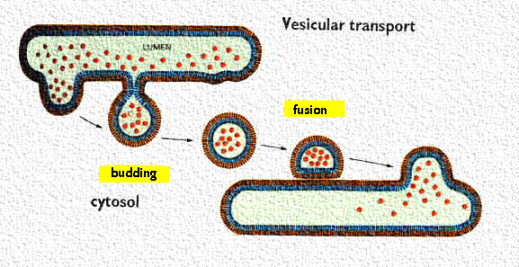
\includegraphics[width=0.6\textwidth]{2.jpg}
\label{fig1}
\end{figure}
In the abstract model of vesicular traffic system compartments are the nodes, and vesicles are the directed edges, of a transport graph. 

\subsection{The model}
The following assumptions reasonably capture the important aspects of the Rothman-Schekman-Sudhof (RSS) model of vesicle traffic.

\begin{enumerate}
\item[1.] A cell is a set of compartments exchanging vesicles.
\item[2.] Compartments are neither created nor destroyed.
\item[3.] Each compartment is in steady state, gain and loss balance.
\item[4.] Molecules are neither created nor destroyed. 
\item[5.] Molecules move via vesicles of uniform size.
\item[6.] Identical vesicles have identical target compartments.
\item[7.] Fusion of vesicles to compartments is driven by specific SNARE pairing.
\item[8.] The activity of a SNARE can be regulated by other molecules present on the same compartment or vesicle.
\item[9.] An active SNARE pair is necessary and sufficient for fusion.
\end{enumerate}

Self loops are not allowed. 

\subsection{Biological model overview}
Let us assume there are M molecular types in the system. These include SNARE proteins, but also include their regulators, and structural molecules such as lipids. Each compartment is a node, specified by an M-length vector giving the amount of various molecular types it contains. Each vesicle is an edge connecting one compartment to another, specified by an M-length vector giving the flux of each molecular type. For this graph to be in steady state, the total incoming and outgoing flux of each molecular type must balance at every node (Fig 2). We assume throughout that self-edges are not permitted (biologically, this could be justified by efficiency considerations).


\begin{figure}[!h]
\centering
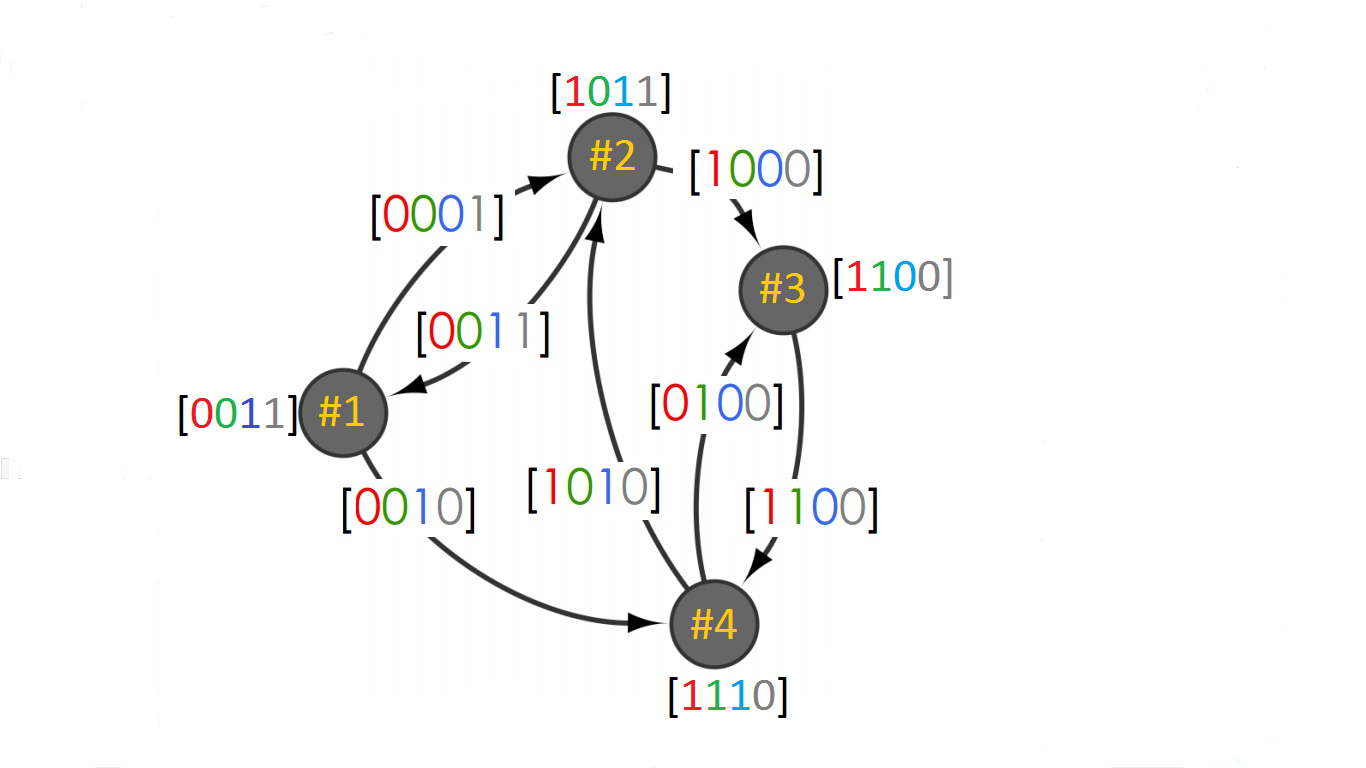
\includegraphics[width=0.75\textwidth]{5.png}
\caption{{\bf The vesicle traffic graph in steady state.} Nodes (large circles) are compartments; vesicles are associated with directed edges. The binary labels represent the presence/absence of four molecular types in this example. The actual amounts of these molecules on each compartment, and actual fluxes along each vesicle edge, can be positive real numbers. By construction, the total incoming flux can be made to balance the total outgoing flux of each molecular type at every node. Note that no pair of vesicles has the identical composition, yet all molecular components move in closed cycles. This is related to the fact that this graph is 3-connected.}
\end{figure}

We next have to specify precisely how SNAREs prefer to pair with one-another, and how the activity of these molecules might be regulated by other molecules in the system. We assume M/2 Q-SNARE types and M/2 R-SNARE types. Fusion is defined by an $M\times M$ binary SNARE pairing matrix, where each non-zero entry states that the corresponding Q-SNARE and R-SNARE pair is fusion competent (Fig 2A,C). The rows/columns represent SNAREs on vesicles/compartments respectively. There are only non-zero entries for Q-R or R-Q pairs. We assume that, due to size and curvature differences, the behavior of molecules on vesicles can be distinct from their behavior on compartments; the matrix is therefore not necessarily symmetric. Rather than invoking further molecular types, we assume the most general situation in which each molecule can take on SNARE-based fusion roles as specified above, or additional regulatory roles. Non-SNARE molecules in this format are those that do not participate in fusion (have no corresponding non-zero entries in the SNARE pairing matrix) but do influence the activity of other SNAREs as described below. Molecules that are to be involved in both fusion and regulation could represent two real molecular types that are always co-localized. This representation is therefore without loss of generality. 

We determine all possible topologies of steady-state vesicle traffic networks that are consistent with models of SNARE regulation.
\begin{figure}
\centering
  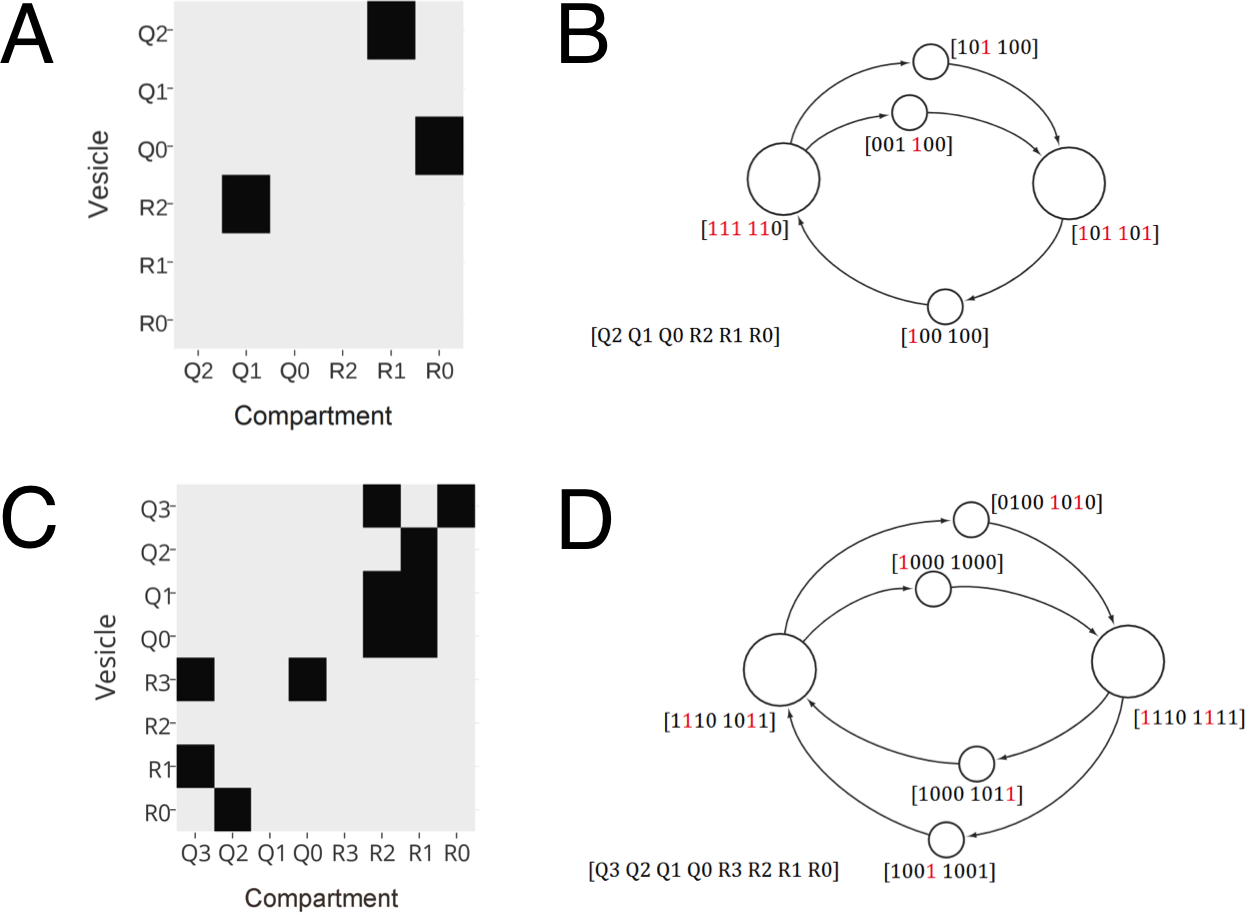
\includegraphics[width=0.85\textwidth]{1.png}
\caption{\textbf{SNARE pairing matrices and the resulting steady state vesicle traffic networks.} SNARE interactions generate the vesicle traffic network. (A,C) Examples of SNARE pairing matrices. Q0, Q1, etc. are Q-SNAREs, R0, R1, etc. are R-SNARES. Dark squares represent SNARE pairings that result in fusion. Each column represents a SNARE type on compartments (nodes), and each row represent a SNARE type on vesicles (edges). SNAREs can be active or inactive depending on the other molecules present on the same vesicle or compartment. If at least one active Q-SNARE type on one membrane interacts with at least one active R-SNARE type on the opposite membrane, compartment-vesicle fusions will occur. (B,D) Steady state vesicle traffic networks governed by SNARE pairings. Nodes (large circles) are compartments; vesicles (small circles) are associated with directed edges. As in Fig 2, we only show the presence or absence of each molecular type on each compartment or vesicle: the first half of the binary vector represents Q-SNAREs, and the second half represents R-SNAREs. The actual fluxes can be positive real numbers, values of which can always be found in order to keep the system in steady state. Active SNAREs are shown in red, inactive SNAREs in black. (A,B) The case of Table 1 row 2, where there is no regulation on compartments (all SNAREs are active) but there is Boolean regulation on vesicles (so only those SNAREs shown in red are active). The necessary and sufficient condition for this case is a 3-connected graph. (C,D) The case of Table 1 row 3, where SNAREs on compartments have Boolean regulation, and SNAREs on vesicles are regulated by SNARE-SNARE inhibition (i.e. if pairing-compatible SNAREs exist on the vesicle, they neutralize one another). The necessary and sufficient condition for this case is a 4-connected graph.}
   \label{fig2} 
\end{figure}

We study a hierarchy of models for varying degrees of regulation of SNARE activity (Table 1). In the simplest case, each SNARE is always considered to be constitutively active (no-regulation model). In the most complex case, the activity state of each SNARE could depend on the presence or absence (defined by a logical Boolean function) of all the other molecules on the corresponding vesicle or compartment (Boolean regulation model). Intermediate between these cases are those in which activity is regulated only on the compartment, or only on the vesicle. We also consider a special case, in which regulation on vesicles has a very restricted form. In this case, we assume that if a fusion-competent Q-R SNARE pair is present on a vesicle (i.e. pair with a non-zero entry in any part of the SNARE pairing matrix) then both molecules are rendered inactive. This is motivated by the fact that these two molecules are likely to zip together, and that NSF is not present on vesicles to unzip them. We refer to this version of regulation as SNARE-SNARE inhibition.

\begin{table}[!ht]
%\begin{adjustwidth}{-2.25in}{0in} % Comment out/remove adjustwidth environment if table fits in text column.
\centering
\def\arraystretch{1.6}
\caption{
{\bf SNARE regulation and graph connectedness.}}
  \begin{tabular}{|c|l|l|c|c|}
    \hline
  \multirow{2}{*}{\textbf{Sr.No}}  & \multirow{2}{*} {\bf{Regulation on compartment}} & \multirow{2}{*} {\bf{Regulation on vesicle}} & \multicolumn{2}{c|}{\textbf{Required graph connectivity}}  \\
    % \hline
    % \textbf{Inactive Modes} & \textbf{Description}\\
    \cline{4-5}
    {} & {} & {} & \textbf{\textbf{Necessary}} & \textbf{Sufficient}\\
    %\hhline{~--}
    \hline
1. & Boolean function & Boolean function & 2-connected & 3-connected \\ \hline
2. & None & Boolean function & 3-connected & 3-connected \\  \hline
3. & Boolean function & SNARE-SNARE inhibition & 4-connected & 4-connected \\ \hline
4. & None & SNARE-SNARE inhibition & No graph & No graph \\ \hline
5. & Boolean function & None & No graph & No graph \\ \hline
6. &  None & None & No graph & No graph \\ \hline
  \end{tabular}
\label{table1}
\end{table}

\section{Formula variables}
Basic notation for the formula we are trying to generate.
\begin{enumerate}
\item edge = e(i,j,q)
      There is an qth edge between node i and j.
      
\item dump = d(i,j,q)
       drop edge(i,j,q) from the graph. 
       
\item presence node = n(i,k) 
	  kth molecule is present on the node i.
      
\item active\_node = a(i,k) 
      kth molecule is active on the node i.
      
\item presence\_edge = e(i,j,q,k)
      There is an qth edge between node i and j with kth molecule present.

\item active\_edge = b(i,j,q,k)
      There is an qth edge between node i and j with kth molecule active.

\item reachability = r(i,j,k,z)
      Node i and j are reachable with kth molecule present in z steps.

\item pairing matrix = p(k,k')
      Molecule k and k' are pairing molecules in the matrix.

\item Type of the Boolean function = sorts (takes k-1 arguments Bool and return Bool) 
\item Boolean function on nodes Function (fn\_{m},*sorts) 

\item Boolean function on edge Function(fe\_{m},*sorts)

\end{enumerate}

\section{Regulation on nodes and edges}
Regulation of a model is based on the kind of the model under consideration. for example model 1 (-V 1) has two different arbitrary Boolean function dictating the activity of the molecules on edge and nodes and for variation 3 (-V 3) activity on edge is driven by SNARE-SNARE inhibition.  

We have build constraints A0, A1 for these two regulations. \newline

A0: No regulation on nodes.
\[ \bigwedge\limits_{i,k} n_{i,k} == a_{i,k} \, \]  

A1: No regulation on edges.
\[ \bigwedge\limits_{i,j,q,k} e_{i,j,q,k} == b_{i,j,q,k} \, \]  

A0: Boolean regulation on nodes. Activity of a molecule k on a node is defined as a Boolean function of presence of other molecule present on that node.
\[ \bigwedge\limits_{i,k} n_{i,k} \supset a_{i,k} ==   f_n[k] (\bigvee_{ k' != k} n_{i,k'}) \, \]  

A1: Boolean regulation on edges. Activity of a molecule k on a node is defined as a Boolean function of presence of other molecule present on that node.
\[ \bigwedge\limits_{i,j,q,k} e_{i,j,q,k} \supset b_{i,j,q,k} == f_e[k](\bigvee_{k' != k} e(i,j,q,k')) \, \]  

A1: SNARE-SNARE inhibition. Inhibition of the edges are driven by the pairing matrix.
\[ \bigwedge\limits_{i,j,i != j, q, k} (\bigwedge_{k' != k} p_{k,k'} \supset e_{i,j,q,k'}) \supset \neg b(i,j,q,k)) \, \]  

\[ \bigwedge\limits_{i,j,i != j, q, k} \neg [(\bigwedge_{k' != k} p_{k,k'} \supset e_{i,j,q,k'})] \supset b(i,j,q,k)) \, \]  

\section{Basic constraints on the edges and nodes}
The edge labels are subset of the node label of source and target compartment. \newline

C0: The edge labels are subset of the node label of source compartment.

\[ \bigwedge\limits_{i,j,k} e_{i,j,k} \supset a_{i,k} \, \]  

C1: The edge labels are subset of the node label of target compartment.

\[ \bigwedge\limits_{i,q}  e_{i,j,k} \supset a_{j,k} \, \]  
%C1 =  e_ijk -> aik and e_ijk -> ajk

C2: Self edges are not allowed. 

\[  \bigwedge\limits_{i,q} \neg e_{i,i,q} \, \]

C4: Condition on p\_kk'. Diagonal blocks should be all 0's.

\[ \bigwedge\limits_{(x < M/2 \, \land  \, y < M/2) \lor  (x >= M/2 \land y >= M/2)} \neg p(x,y) \, \]

C5: Activity on the node. A molecule should be present to be active on a node.  
\[ \bigwedge\limits_{i,k} a_{i,k} \supset n_{j,k} \, \]  

% - F0: b(i,j,k) $\supset$ e(i,j,k)



\section{Main constraints}
Main constraints to be followed. \newline

F0:  An edge has to have one present molecule. F0 looks redundant.

\[ \bigwedge\limits_{i,j,q} \bigvee_k e_{i,j,q,k} \supset e_{i,j,q} \, \]  

F1: If molecule is active on an edge then it should be present on the edge.

\[ \bigwedge\limits_{i,j,q,k} a_{i,j,q,k} \supset e_{i,j,q,k}\, \]



\section{Steady state specification}
Each molecule leaving the node on a vesicle should come back to its source node in a cycle, i.e., \textbf{for every molecule leaving the node there exists a cycle with that molecule present on \textit{each of the edges and nodes} of the path taken}.

\subsection{Reachability definition and stability condition}
If molecule is active on an edge then it should be present on the edge. \newline


F3: stability condition. Source node is reachable by target node with that molecule present in p steps.

% I have implemented: Changed the implementation in code too.
%\[ \bigwedge\limits_{i,j,q,k} e_{i,j,q,k} \supset (r_{j,i,k,0}  \lor r_{j,i,k,1} \lor ... \lor r_{j,i,k,p}) \, \]

% Update: Better 
\[ \bigwedge\limits_{i,j,k} (\bigvee_{q} e_{i,j,q,k}) \supset (r_{j,i,k,0}  \lor r_{j,i,k,1} \lor ... \lor r_{j,i,k,p}) \, \]

F2: Reachability definition.
\[ \bigwedge\limits_{i,j,k,p} r_{i,j,k,p} \supset (\bigvee_{q} \, e_{i,j,q,k} \lor \bigvee_{i\neq i^{\prime}} ( \, \bigvee_{q} e_{i,i^{\prime},q,k}) \land r_{i^{\prime},j,k,p-1} ) \, \]


\section{ Fusion rule Formula}

Fusion rules consist of two different mechanisms.

\begin{enumerate}
\item  A \textbf{SNARE pairing mechanism} which determines compatible Q-R pairs on vesicles and compartments that can cause fusion.
\item \textbf{Regulatory mechanisms} on edges and on nodes (possibly distinct) which regulate SNARE activity based on the presence/absence of other molecules on the corresponding node or edge.
\end{enumerate}

F4: For an edge to be valid, at least one SNARE pair on the vesicle and target compartment must be active, and have a non-zero entry in the pairing matrix.  

\[ \bigwedge\limits_{i,j,q} e_{i,j,q} \supset \bigvee_{k,k^{\prime}} (b_{i,j,q,k} \land a_{j,k^{\prime}} \land p_{k,k^{\prime}}) \, \]

F5: To ensure that fusion respects the graph structure by the edge under consideration, it should not be possible to fuse with any other node.

\[ \bigwedge\limits_{i,j,k} b_{i,j,k} \supset \neg \bigvee_{j \neq j^{\prime}, k^{\prime\prime}} ( a_{j^{\prime},k^{\prime\prime}} \land p_{k,k^{\prime\prime}}) \, \]


\section{Connectivity}
To check the whether that n connected is necessary condition, we remove (drop) n edges from the graph and if it disconnects the graph and we get an assignment we have a n connected satisfying graph. We can go down or up using -C \_ option.  \newline 

D0: Only present edges can be dropped.
\[ \bigwedge\limits_{i,j,q} d_{i,j,q} \supset e_{i,j,q}  \]

D1,D2: We are dropping c edges from the graph. exactly c are dropped.
\[ \sum_{i,j,q} d_{i,j,q} == c \]

D3:  Graph becomes disconnected. Ensure that there is no path between some nodes i,j in the underlying undirected graph. Different reachability.
\[ \bigwedge\limits_{i,j} \neg (r^{\prime}_{i,j} \lor r^{\prime}_{j,i})]  \]

D4: New reachability definition for grph connectedness: dReachable. Node i,j are reachable either if there is a direct edge and its not dropped. 
Or there is an node i' such that, there is a direct edge between i,i' which is not dropped and i' and j is dReachable.

\[ \bigwedge\limits_{i,j}  [\bigvee_{q} (e_{i,j,q} \land  \neg d_{i,j,q}) \lor  (\bigvee_{i' != i}  r^{\prime}(i',j) \land  \bigvee_{q} (e_{i,i',q} \land \neg d_{i,i',q}) ] \supset r^{\prime}(i,j)  \]
  
\end{document}